\section{Results}
\label{sec:results}

This section presents the main results of the FRESNEL field campaign,
focusing on the integration of model forecasts, target sampling, and
data assimilation using autonomous underwater vehicles (AUVs). The
analysis combines CMS and statistical model forecasts (as described
in the Methods section) with in situ observations to assess how the
proposed data-cycle approach can enhance short-term ocean prediction
in a dynamic coastal environment.

Fig. \ref{fig:sst} provides an overview of the environmental
conditions observed during the three-day experimental window
considered in this study (29–31 October). The background fields
correspond to the Level-3 Sea Surface Temperature (SST) product from
Copernicus Marine Service (\url{DOI:10.48670/moi-00310})

Following the overview of the surface conditions, Figure \ref{fig:temperatureprofiles} presents the vertical temperature distribution recorded by the LAUVs XP2, XP3, and XP5 during their respective missions between 29 and 31 October. The panels show temperature as a function of time and depth, illustrating the temporal and vertical structure of the coastal water column throughout the three-day experimental sequence.

XP2 operated on 29 October, XP5 on 29, 30, and 31 October, and XP3 on 30 and 31 October, with all vehicles capable of sampling the upper 100 m of the water column. However, this depth range was not always achieved due to logistical and bathymetric constraints. The temperature fields reveal a thermocline and a progressive warming of the surface layer down to approximately 40 m depth, with temperatures ranging from around 14 °C in deeper layers to about 18 °C near the surface, reaching their maximum on 30 October afternoon during XP5’s mission.

It is important to note that the trajectories shown in the previous figure might suggest that the AUVs remained continuously at sea for 24 hours each day. However, as Figure \ref{fig:temperatureprofiles} demonstrates, this was not the case. The vehicles can be deployed and recovered multiple times per day, with operational windows limited by logistics, weather, and available support assets. This figure, therefore, also highlights the non-linear nature of field logistics in multi-vehicle operations, where dynamic scheduling, resource allocation, and environmental constraints determine the actual temporal coverage of the missions.

\begin{figure}
  \centering \subfigure[Sea surface temperature (SST) and XP2, XP3 and XP5 trajectories during the FRESNEL field campaign (29–31 October).]{\label{fig:sst}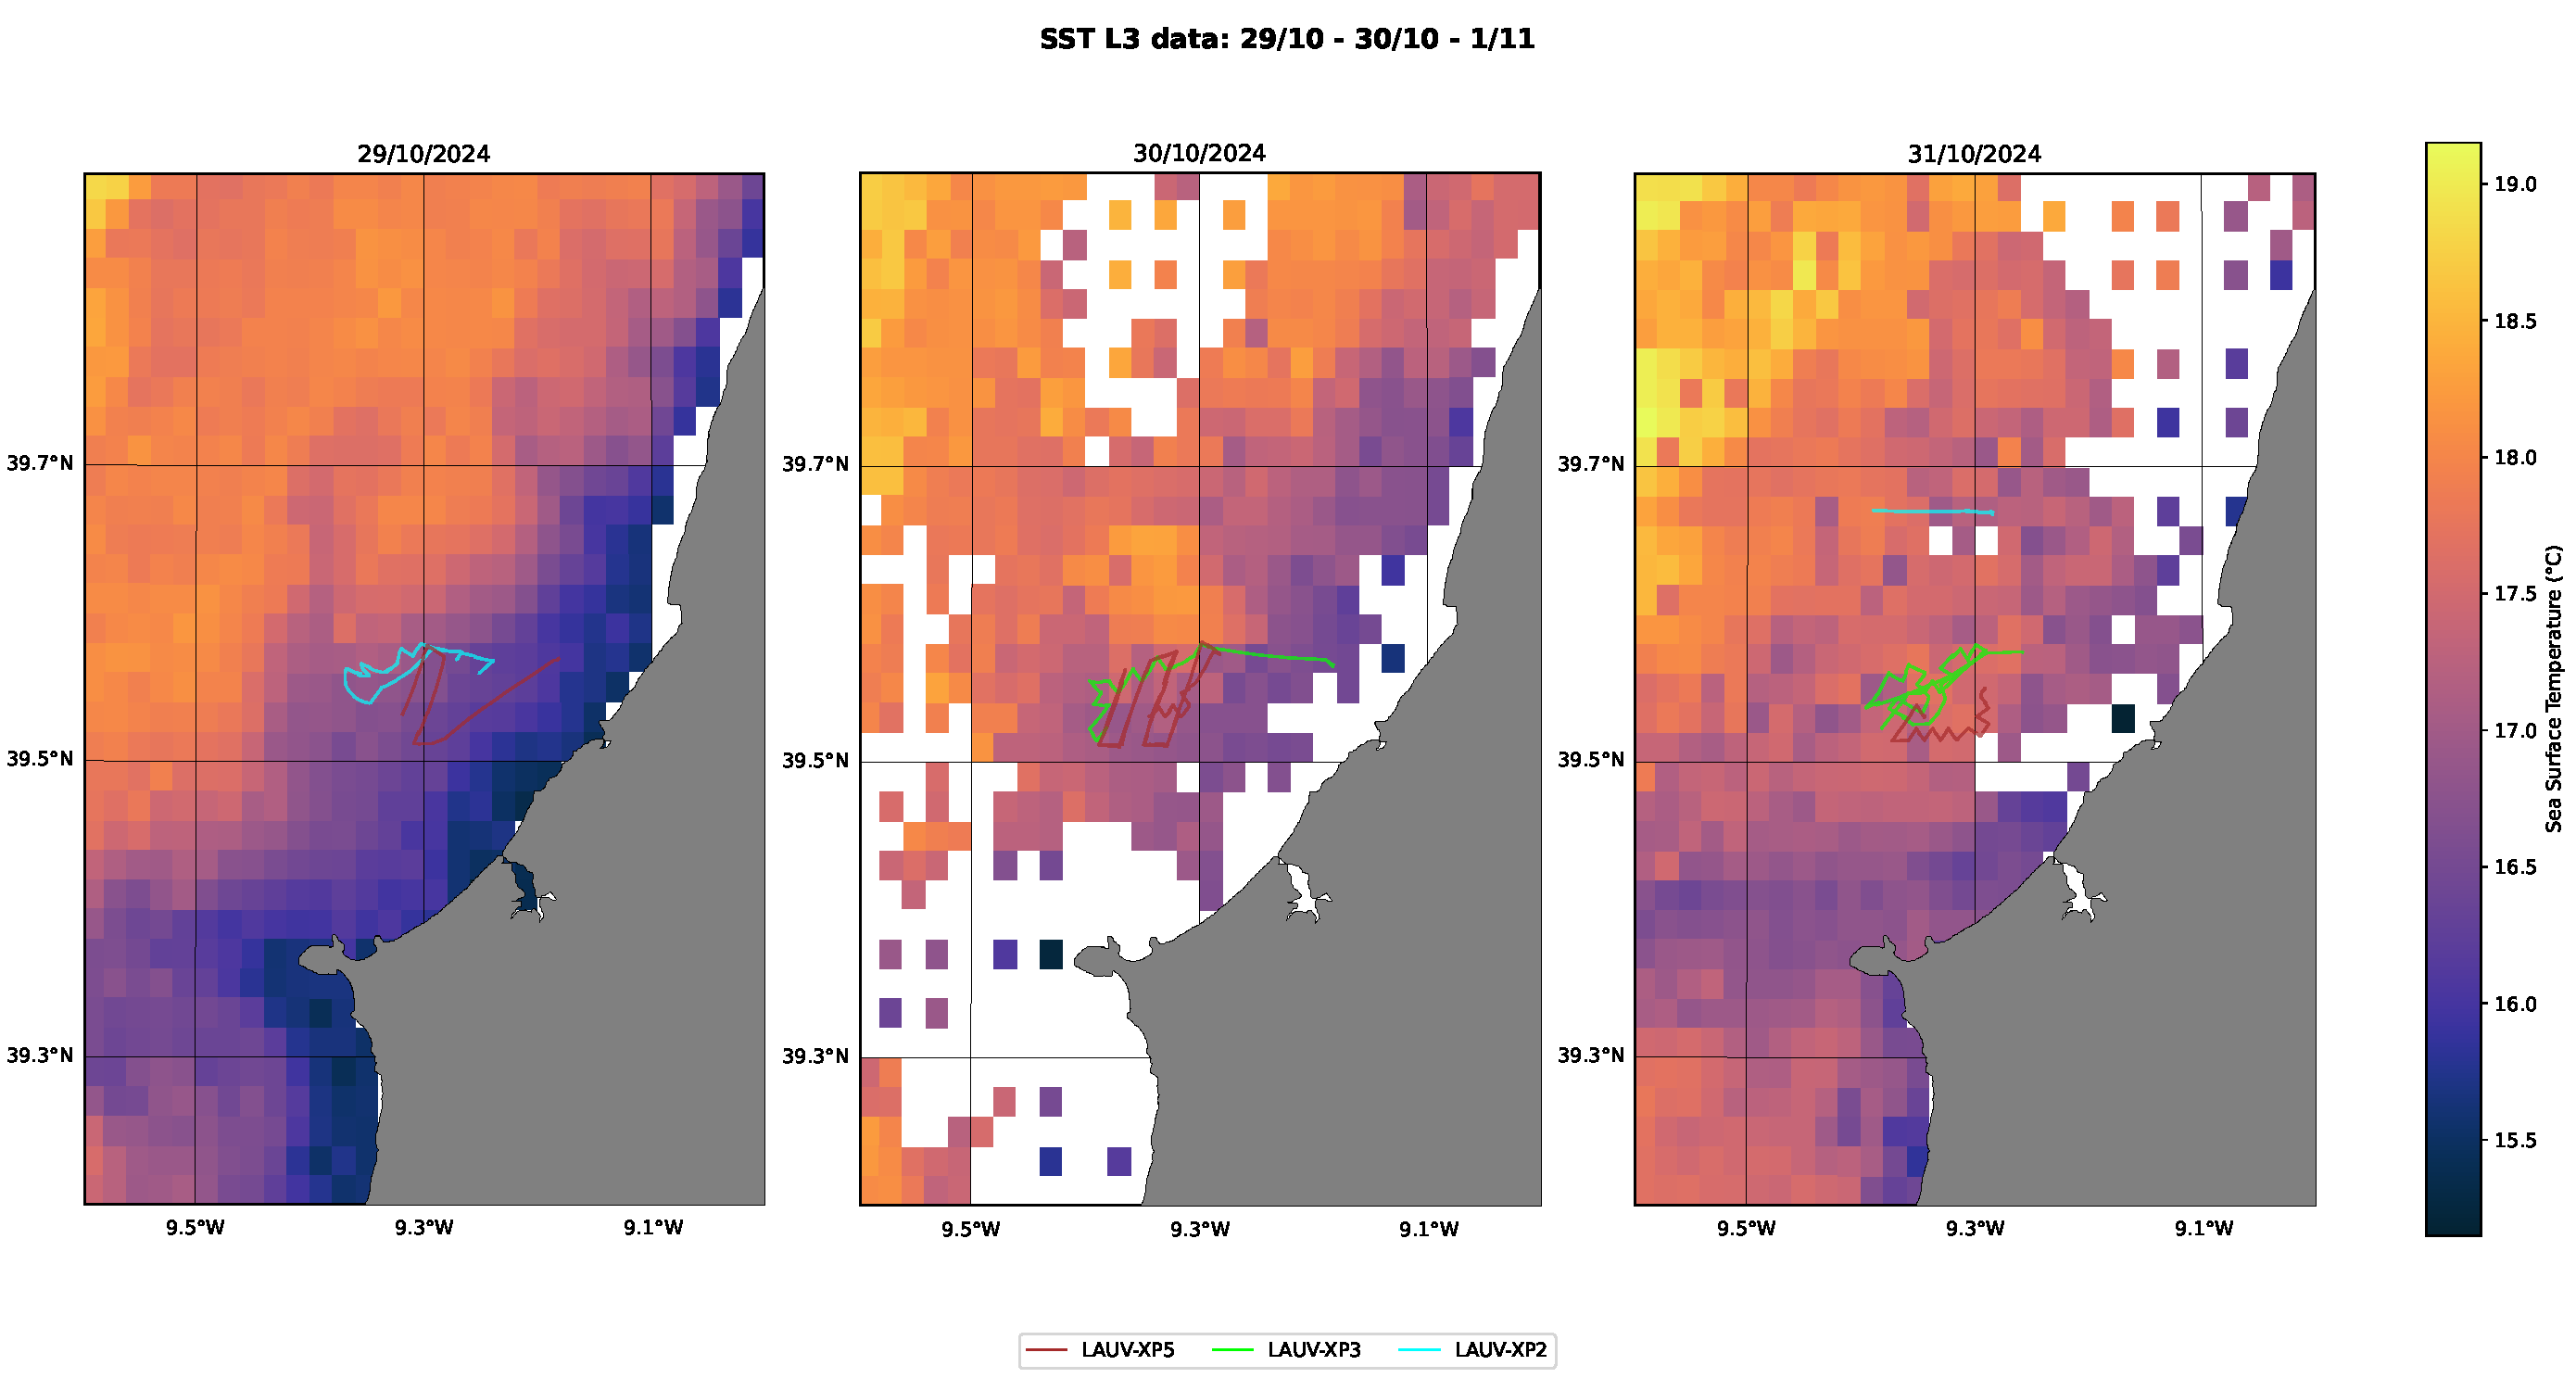
\includegraphics[width=1\linewidth]{fig/SST_L3_color1.pdf}}
  \subfigure[Time–depth temperature evolution observed by XP2, XP3, and XP5 during the FRESNEL field campaign (29–31 October).]{\label{fig:temperatureprofiles}\includegraphics[width=1\linewidth]{fig/Figure2_100m.pdf}}
\end{figure}

\begin{itemize}
    \item Environmental context
    \item RMS table (all cases) + rms figure (just A+D cases)
\end{itemize}

 
\textit{- Use \textbf{subheadings} to organize different experiments or analyses.}
